\documentclass[11pt,a4paper]{article}

\usepackage[T1]{fontenc}
\usepackage[utf8]{inputenc}
\usepackage{lmodern}
\usepackage{microtype}
\usepackage[margin=2.4cm]{geometry}
\usepackage{amsmath,amssymb,amsthm,mathtools}
\usepackage{booktabs,array,tabularx}
\usepackage{graphicx}
\usepackage[dvipsnames]{xcolor}
\usepackage{tikz}
\usetikzlibrary{arrows.meta,positioning,calc,decorations.pathreplacing}
\usepackage[ruled,vlined,linesnumbered]{algorithm2e}
\usepackage{enumitem}
\usepackage{caption}
\usepackage[backend=bibtex,style=numeric-comp,sorting=nyt,maxbibnames=6,giveninits=true,doi=true,url=false]{biblatex}
\addbibresource{refs.bib}
\usepackage[colorlinks=true,linkcolor=NavyBlue,citecolor=ForestGreen,urlcolor=NavyBlue]{hyperref}
\usepackage[capitalise,nameinlink]{cleveref}

\definecolor{cblue}{HTML}{2A78D6}
\definecolor{corange}{HTML}{EB6834}
\definecolor{caqua}{HTML}{1BAF7A}
\definecolor{cgray}{HTML}{8A8984}
\definecolor{ours}{HTML}{E8F1FB}

\theoremstyle{plain}
\newtheorem{theorem}{Theorem}
\newtheorem{proposition}[theorem]{Proposition}
\newtheorem{lemma}[theorem]{Lemma}
\newtheorem{corollary}[theorem]{Corollary}
\newtheorem{observation}[theorem]{Observation}
\theoremstyle{definition}
\newtheorem{definition}[theorem]{Definition}
\newtheorem{example}[theorem]{Example}
\newtheorem{remark}[theorem]{Remark}
\crefname{observation}{Observation}{Observations}
\Crefname{observation}{Observation}{Observations}

\newcommand{\F}{\mathbb{F}}
\newcommand{\Ftm}{\F_{2^m}}
\newcommand{\Red}{\operatorname{Red}}
\newcommand{\dX}{\operatorname{dXOR}}
\newcommand{\CX}{\operatorname{CX}}
\newcommand{\xor}{\oplus}
\newcommand{\ours}{\textsuperscript{\textcolor{cblue}{$\blacklozenge$}}}
\SetKwInOut{Input}{Input}\SetKwInOut{Output}{Output}

\title{\textbf{Efficient Closed-Form Reduction for Banegas’ Second Family of Pentanomials}}
\author{Marcos Tomaszewski \and Ricardo Custódio \and Gustavo Banegas \and Daniel Panario \\[4pt]
\small Laboratório de Segurança em Computação (LabSEC)\\
\small Departamento de Informática e Estatística, Universidade Federal de Santa Catarina\\
\small Florianópolis, SC, Brazil}
\date{}

\begin{document}
\maketitle

\begin{abstract}

In polynomial-basis arithmetic over \(\mathbb{F}_{2^m}\), the choice of the defining irreducible polynomial directly affects the cost of modular reduction and, consequently, the implementation cost of field multiplication. Using a greedy XOR-counting heuristic, Banegas identified two families of low-cost pentanomials. The first family was subsequently analysed by Banegas, Custódio, and Panario, whereas the second family,
\[
f_{b,c}(x)=x^{b+2c}+x^{b+c}+x^b+x^c+1,
\qquad b>c\ge1,
\]
was left as an open direction because of its more involved reduction structure.

In this work, we provide a formal analysis of this second family. For \(m=b+2c\), we derive a closed-form expression for the quotient arising in polynomial reduction, expressed through comb sums of stride \(3c\), and use it to construct an explicit reduction circuit requiring at most \(3m-c-3\) XOR gates, with depth at most
\[
\left\lfloor\frac{m-2}{3c}\right\rfloor+4.
\]
Combined with a schoolbook polynomial multiplier, the construction yields a bit-parallel multiplier using \(m^2\) AND gates and \(m^2+m-c-2\) XOR gates, of which \((m-1)^2\) are spent on the product and \(3m-c-3\) on the reduction. For admissible parameters with \(c\) close to \(m/3\), the reduction bound approaches \(8m/3\) XOR gates.

We symbolically verified the reduction construction for all 14,850 members with \(m\le300\). An irreducibility census for \(5\le m\le1100\) found members of the second family in 720 degrees, including 288 degrees for which no irreducible trinomial exists. Among the 405 degrees containing irreducible members of both Banegas families, the best member of the second family has a lower reduction bound in 403. At the NIST binary-field degrees 163 and 571, the best members found in the second family require 440 and 1,528 XOR gates, respectively, compared with the reported counts of 571 and 2,003 for the corresponding NIST pentanomials; at
degree 283, the remaining NIST pentanomial degree, the second family has no irreducible member.

\medskip\noindent\textbf{Keywords:} binary finite fields; irreducible pentanomials; modular reduction; XOR circuit complexity; bit-parallel multipliers; polynomial basis
\end{abstract}

% ==================================================================
\section{Introduction}\label{sec:intro}
% ==================================================================

\paragraph{Finite field arithmetic.}
Finite fields are the algebraic substrate of most cryptographic primitives and of many
error-correcting codes \cite{LidlNiederreiter1997,HMV2004}. Two kinds of fields dominate
implementations. \emph{Prime fields} $\F_p$ with a large prime $p$ use multiprecision
integer arithmetic, and special primes make modular reduction cheap. \emph{Binary
extension fields} $\Ftm\cong\F_2[x]/(f)$, with $f$ irreducible of degree $m$, use
carry-free arithmetic: addition is a bitwise XOR and multiplication is a carry-less
product followed by a reduction modulo $f$. Elements can be represented in polynomial,
normal, shifted or Montgomery bases, or as towers of subfields. In the polynomial basis
the product stage does not depend on $f$, while the reduction depends only on $f$;
choosing $f$ is therefore a design decision with a direct effect on area, delay and
energy in hardware and on the instruction count of bitsliced software.

\paragraph{Prime fields in standards, binary fields in practice.}
For elliptic curve cryptography the NIST recommendations moved to prime fields: SP
800-186 keeps the prime-field curves, adds Edwards curves, and deprecates the curves
over binary fields, whose defining polynomials were the trinomials of degrees $233$ and
$409$ and the pentanomials of degrees $163$, $283$ and $571$ \cite{SP800186,FIPS1865}.
Binary fields in polynomial basis nevertheless remain in daily use: the AES operates in
$\F_{2^8}$ \cite{FIPS197}; GCM authenticates with a pentanomial of degree $128$
\cite{SP80038D,GueronKounavis2010}; Classic McEliece computes in $\F_{2^{12}}$ and
$\F_{2^{13}}$ \cite{ClassicMcEliece2022,McBits2013}; the post-quantum signature scheme
FAEST works in $\F_{2^\lambda}$ \cite{FAEST2023}; succinct arguments use towers of binary
fields \cite{DiamondPosen2025}; and Reed--Solomon and BCH codecs, the motivation of the
classic work of Paar \cite{Paar1997}, still reduce in binary fields. In all these
settings each XOR gate counts.

\paragraph{Special polynomials.}
Trinomials give the cheapest reduction, $2m-2$ XORs \cite{SunarKoc1999,Wu2002}, but no
irreducible trinomial exists for many degrees: none for $m\equiv0\pmod 8$ and none for
many odd $m\equiv\pm3\pmod 8$, as a consequence of Swan's theorem \cite{Swan1962}. For
those degrees one uses pentanomials, and a line of work proposed pentanomial families
with low reduction or multiplication cost
\cite{HasanWangBhargava1992,RodriguezKoc2003,ReyhaniHasan2004,Cilardo2013,Imana2018,BCP2019}.

\paragraph{Banegas' two families.}
In his master's thesis at LabSEC/UFSC, Banegas implemented a greedy XOR counter,
\emph{Conta-XOR}, ran it over all irreducible pentanomials of degrees $19$ and $163$,
and identified two families of pentanomials with small counts \cite{Banegas2015}:
\[
\text{(first)}\quad x^{2b+c}+x^{b+c}+x^b+x^c+1,\qquad\qquad
\text{(second)}\quad x^{b+2c}+x^{b+c}+x^b+x^c+1 .
\]
The first family was analysed by Banegas, Custódio and Panario (BCP): the reduction
costs $3m-2$ XORs, and $\tfrac{12}{5}m-1$ when $b=2c$ \cite{BCP2019}. About the second,
the thesis states that it ``demonstrated that a greater understanding of the reduction
process that involves it is necessary'' (our translation) and proposes its study as future work
\cite[Sec.~4.5]{Banegas2015}. Ten years later, this paper carries out that study.

\paragraph{Contributions.}
Results marked \ours{} are new; every other result is cited.
\begin{enumerate}[leftmargin=*,itemsep=2pt]
  \item \ours{} Structural facts about the second family, including the identity
        $(x^c+1)f=x^{b+3c}+x^b+x^{2c}+1$, which drives everything else
        (\cref{sec:family}).
  \item \ours{} A closed form for the quotient $\lfloor D/f\rfloor$ in terms of comb
        sums of stride $3c$ (\cref{thm:quotient}).
  \item \ours{} An explicit reduction program with at most $3m-c-3$ XORs and depth at
        most $\lfloor(m-2)/3c\rfloor+4$, for all $b>c\ge1$, and the corresponding
        multiplier with $m^2+m-c-2$ XORs (\cref{thm:main,prop:depth,cor:mult}).
  \item \ours{} A word-level formulation with $O(\log(m/c))$ shift-and-XOR operations,
        and a low-depth gate-level variant (\cref{sec:word}).
  \item \ours{} A comparison with the Conta-XOR count: the closed form is never worse
        on generic members, it explains the counts reported in the thesis, and it
        improves on them by exactly $2c-b$ when $b<2c$ (\cref{sec:greedy}).
  \item \ours{} A census of irreducible members up to degree $1100$ and a comparison
        with the first family, with trinomials and with the NIST pentanomials
        (\cref{sec:comparison}).
\end{enumerate}

% ==================================================================
\section{Background}\label{sec:background}
% ==================================================================

We recall the notation and known results used in the rest of the paper.

\subsection{Reduction and its cost}

Let $f=x^m+g$ with $g(0)=1$ and $\deg g<m$. The product of two elements of $\Ftm$ is
$D=\sum_{j=0}^{2m-2}d_jx^j$, which we split as
\begin{equation}\label{eq:split}
  D=L+x^mH,\qquad L=\sum_{i=0}^{m-1}d_ix^i,\qquad H=\sum_{s=0}^{m-2}h_sx^s,\quad h_s=d_{m+s}.
\end{equation}
Reduction computes $R=D\bmod f$. It is a fixed $\F_2$-linear map: the \emph{reduction
matrix} $R_f\in\F_2^{m\times(2m-1)}$ has as column $j$ the coefficients of
$x^j\bmod f$, and $R=R_f\,(d_0,\dots,d_{2m-2})^{\top}$. A \emph{linear straight-line
program} computes $R$ with instructions $t\gets u\xor v$ over inputs and earlier
results; its length is the number of XOR gates, and its \emph{depth} is the length of the
longest chain of dependent gates. The \emph{direct count}
$\dX(f)=\sum_i(\text{weight of row }i-1)$ adds each output from scratch. We write
$\Red(f)$ for the minimum length of a program for $R_f$. Computing $\Red(f)$ is NP-hard
in general \cite{BMP2013}; heuristics include the greedy algorithm of Paar, which
repeatedly replaces the most frequent pair of operands by a new variable
\cite{Paar1997}, the heuristic of Boyar and Peralta, which allows cancellations
\cite{BoyarPeralta2010}, and their many refinements
\cite{Kranz2017,Banik2019,TanPeyrin2020,Xiang2020,SunYangLi2025}. Exact values are
obtained with SAT solvers for small instances \cite{FuhsSK2010,Stoffelen2016}.

\subsection{Conta-XOR}

Conta-XOR \cite[Ch.~4]{Banegas2015} builds a reduction matrix by repeated substitution
of $x^m$ by $g$, removes pairs of equal terms in each output, replaces repeatedly the most
repeated pair of operands by a temporary variable, and reports the number of temporaries
plus the remaining additions. We write $\CX(f)$ for its value, which we recomputed with
an independent implementation that reproduces the values published in
\cite{Banegas2015}; ties between equally frequent pairs are broken lexicographically.

\subsection{Known special pentanomials}

\Cref{tab:known} lists closed-form reduction costs from the literature for the special
polynomials we compare with.

\begin{table}[t]
\centering\small
\caption{Reduction costs of special irreducible polynomials (literature).}
\label{tab:known}
\begin{tabular}{@{}l l l l@{}}
\toprule
Polynomial & Condition & XORs for reduction & Ref.\\
\midrule
trinomial $x^m+x^k+1$ & $k\le m/2$ & $2m-2$ & \cite{SunarKoc1999,Wu2002}\\
equally spaced $x^{4c}+x^{3c}+x^{2c}+x^c+1$ & $m=4c$ & $\tfrac74m-1$ & \cite{HasanWangBhargava1992,Banegas2015}\\
Banegas' first family $x^{2b+c}+x^{b+c}+x^b+x^c+1$ & $b>c$ & $3m-2$ & \cite{BCP2019}\\
\quad the same, with $b=2c$ & $m=5c$ & $\tfrac{12}{5}m-1$ & \cite{BCP2019}\\
\bottomrule
\end{tabular}
\end{table}

For a schoolbook product the partial products cost $m^2$ AND gates and $(m-1)^2$ XOR
gates, so a multiplier costs $(m-1)^2$ plus the reduction; for the first family this is
$m^2+m-1$ XORs \cite{BCP2019}.

% ==================================================================
\section{The second family}\label{sec:family}
% ==================================================================

\begin{definition}\label{def:family}
For integers $b>c\ge1$ let $m=b+2c$ and
\[
  f_{b,c}(x)=x^{b+2c}+x^{b+c}+x^b+x^c+1 .
\]
We call $\{f_{b,c}\}$ \emph{Banegas' second family}, and write $n=m-2$ for the degree of
$H$ in \eqref{eq:split}.
\end{definition}

The constraint $b>c$ is part of the definition in \cite{Banegas2015}; it also guarantees
that the exponents are distinct, because $b+c<b+2c$ and $c<b$.

\begin{proposition}[\ours]\label{prop:basic}
Let $f=f_{b,c}$.
\begin{enumerate}[label=(\roman*),itemsep=1pt]
  \item $x^m\equiv(x^b+1)(x^c+1)\pmod f$.
  \item $(x^c+1)\,f=x^{b+3c}+x^b+x^{2c}+1$, hence $x^b(x^{3c}+1)\equiv(x^c+1)^2\pmod f$.
  \item $1\le c\le\lfloor (m-1)/3\rfloor$ and $b\equiv m\pmod 2$.
  \item If $g=\gcd(b,c)>1$ then $f(x)=G(x^g)$ for the pentanomial $G=f_{b/g,\,c/g}$.
  \item For $b=2c$, $f$ is the equally spaced pentanomial $x^{4c}+x^{3c}+x^{2c}+x^c+1$.
\end{enumerate}
\end{proposition}

\begin{proof}
(i) $x^{b+c}+x^b+x^c+1=(x^b+1)(x^c+1)$. (ii) Expanding,
$(x^c+1)(x^{b+2c}+x^{b+c}+x^b+x^c+1)
=x^{b+3c}+x^{b+2c}+x^{b+2c}+x^{b+c}+x^{b+c}+x^b+x^{2c}+x^c+x^c+1$, and the repeated terms
cancel. Reducing $x^{b+3c}=x^{2c}\cdot x^m$ gives the second statement. (iii) $b>c$ and
$m=b+2c$ give $m>3c$; $m-b=2c$ is even. (iv) and (v) are immediate.
\end{proof}

Identity (ii) is the key to the whole analysis: a shift by $3c$ applied to the high part
can be undone at the price of two low-order terms. The first family has the analogous
identity $(x^b+1)f=x^{3b+c}+x^{2b}+x^c+1$, obtained in the same way, but with a shift of
$b$ instead of $c$; this is one reason why the two families behave differently.

% ==================================================================
\section{A closed form for the quotient}\label{sec:quotient}
% ==================================================================

\begin{lemma}[Division identities]\label{lem:division}
Let $f=x^m+\sum_{e\in S}x^e+1$, $S\subseteq\{1,\dots,m-1\}$, and let $Q=\lfloor D/f\rfloor
=\sum_{j=0}^{n}q_jx^j$. Then
\begin{align}
  h_j &= q_j+\sum_{e\in S} q_{j+m-e}, && 0\le j\le n, \label{eq:high}\\
  r_i &= d_i+\sum_{e\in S\cup\{0\}} q_{i-e}, && 0\le i\le m-1, \label{eq:low}
\end{align}
with $q_k=0$ for $k<0$ or $k>n$.
\end{lemma}

\begin{proof}
This is polynomial long division written coefficientwise: from $D=Qf+R$ and
$f=x^m+g$, compare the coefficients of $x^{m+j}$ ($j\ge0$), where $R$ does not
contribute, and of $x^i$ ($i<m$), where $x^mQ$ does not contribute.
\end{proof}

For the second family $S=\{c,\,b,\,b+c\}$ and $m-S=\{b+c,\,2c,\,c\}$, so \eqref{eq:high}
reads
\begin{equation}\label{eq:rec}
  h_j=q_j+q_{j+c}+q_{j+2c}+q_{j+b+c}.
\end{equation}
Equation \eqref{eq:rec} determines $Q$ from the top down, but evaluating it directly
costs almost one XOR per coefficient of $Q$. The next theorem solves the recurrence.

\begin{definition}[\ours{} Comb sums]
For $t\ge0$ let
\[
  C_t=\sum_{k\ge0,\ t+3ck\le n} h_{t+3ck},
\]
the sum of the high coefficients whose index is congruent to $t$ modulo $3c$ and at
least $t$; $C_t=0$ for $t>n$. Equivalently $C_t=h_t\xor C_{t+3c}$.
\end{definition}

\begin{theorem}[\ours{} Closed-form quotient]\label{thm:quotient}
For $f=f_{b,c}$ and $0\le j\le n$,
\begin{equation}\label{eq:qclosed}
  q_j=C_j+C_{j+c}+h_{j+b+c},
\end{equation}
where $h_s=0$ for $s>n$. Consequently the polynomial $U=(1+x^c)Q$, with coefficients
$U_k=q_k+q_{k-c}$, satisfies
\begin{equation}\label{eq:Uclosed}
  U_k=\begin{cases}
    C_k+C_{k+c}+h_{k+b+c}, & 0\le k<c,\\[2pt]
    C_{k-c}+C_{k+c}+h_{k+b}, & k\ge c,
  \end{cases}
\end{equation}
and the remainder is
\begin{equation}\label{eq:rU}
  r_i=d_i+U_i+U_{i-b}\qquad(0\le i\le m-1;\ U_{i-b}=0 \text{ if } i<b).
\end{equation}
\end{theorem}

\begin{proof}
Define $\tilde q_j$ by the right-hand side of \eqref{eq:qclosed} for all $j\ge0$. Then
$\tilde q_j=0$ for $j>n$, since every index involved exceeds $n$. We show that
$\tilde q$ satisfies \eqref{eq:rec}; since \eqref{eq:rec} determines $q_j$ uniquely from
$q_{j+1},\dots,q_n$, it follows that $\tilde q=q$. Adding the four right-hand sides,
\begin{align*}
\tilde q_j+\tilde q_{j+c}+\tilde q_{j+2c}+\tilde q_{j+b+c}
 &=(C_j+C_{j+c}+h_{j+b+c})+(C_{j+c}+C_{j+2c}+h_{j+b+2c})\\
 &\quad+(C_{j+2c}+C_{j+3c}+h_{j+b+3c})+(C_{j+b+c}+C_{j+b+2c}+h_{j+2b+2c}).
\end{align*}
Since $b+2c=m>n$, the terms $h_{j+b+2c}$, $h_{j+b+3c}$, $h_{j+2b+2c}$ and
$C_{j+b+2c}$ vanish. The pairs $C_{j+c}$ and $C_{j+2c}$ cancel. Finally
$C_{j+b+c}=h_{j+b+c}$, because $j+b+c+3c>n$; both sides are zero when $j+b+c>n$. The sum
therefore equals $C_j+C_{j+3c}=h_j$, which is \eqref{eq:rec}.

For \eqref{eq:Uclosed}: if $k<c$ then $q_{k-c}=0$ and $U_k=q_k$. If $k\ge c$, then
$U_k=q_k+q_{k-c}=(C_k+C_{k+c}+h_{k+b+c})+(C_{k-c}+C_k+h_{k+b})$; the term $h_{k+b+c}$
vanishes because $k+b+c\ge b+2c>n$, and $C_k$ cancels. Finally \eqref{eq:low} with
$S=\{c,b,b+c\}$ gives
$r_i=d_i+(q_i+q_{i-c})+(q_{i-b}+q_{i-b-c})=d_i+U_i+U_{i-b}$.
\end{proof}

\begin{figure}[t]
\centering
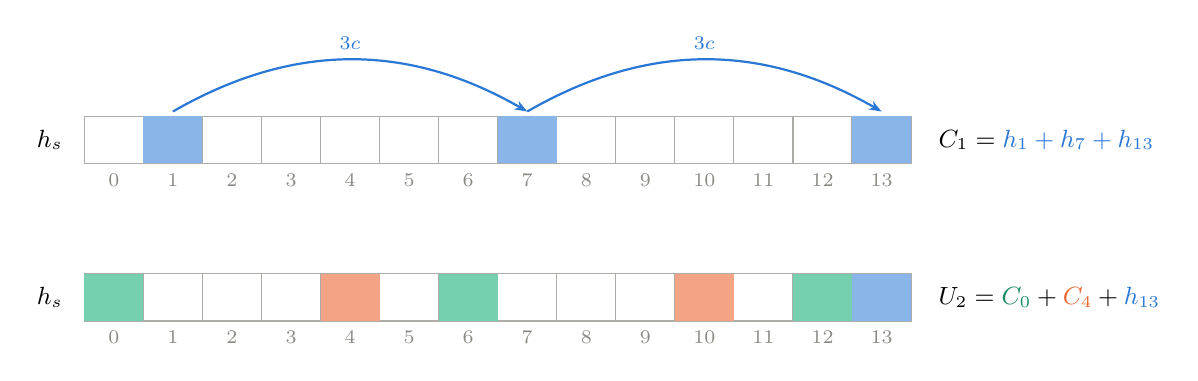
\begin{tikzpicture}[x=7.5mm,y=6mm,every node/.style={font=\small}]
  \foreach \s in {0,...,13}{\draw[cgray!70] (\s,0) rectangle (\s+1,1); \node[font=\scriptsize,cgray] at (\s+0.5,-0.35) {\s};}
  \node[anchor=east] at (-0.2,0.5) {$h_s$};
  \foreach \s in {1,7,13}{\fill[cblue!55] (\s,0) rectangle (\s+1,1);}
  \draw[cblue,thick,-{Stealth[length=1.6mm]}] (1.5,1.1) to[bend left=30] node[above,font=\scriptsize]{$3c$} (7.5,1.1);
  \draw[cblue,thick,-{Stealth[length=1.6mm]}] (7.5,1.1) to[bend left=30] node[above,font=\scriptsize]{$3c$} (13.5,1.1);
  \node[anchor=west] at (14.3,0.5) {$C_1=\textcolor{cblue}{h_1+h_7+h_{13}}$};
  \begin{scope}[yshift=-20mm]
  \foreach \s in {0,...,13}{\draw[cgray!70] (\s,0) rectangle (\s+1,1); \node[font=\scriptsize,cgray] at (\s+0.5,-0.35) {\s};}
  \node[anchor=east] at (-0.2,0.5) {$h_s$};
  \foreach \s in {0,6,12}{\fill[caqua!60] (\s,0) rectangle (\s+1,1);}
  \foreach \s in {4,10}{\fill[corange!60] (\s,0) rectangle (\s+1,1);}
  \fill[cblue!55] (13,0) rectangle (14,1);
  \node[anchor=west,align=left] at (14.3,0.5) {$U_2=\textcolor{caqua!80!black}{C_0}+\textcolor{corange}{C_4}+\textcolor{cblue}{h_{13}}$};
  \end{scope}
\end{tikzpicture}
\caption{\ours{} Comb sums and the closed form \eqref{eq:Uclosed}, for $b=11$, $c=2$
($m=15$, $n=13$, stride $3c=6$). Top: the comb sum $C_1$. Bottom: $U_2=C_{0}+C_{4}+h_{13}$,
the sum of two comb sums and one extra high coefficient ($k=2\ge c$, so $C_{k-c}=C_0$,
$C_{k+c}=C_4$ and $h_{k+b}=h_{13}$).}
\label{fig:comb}
\end{figure}

% ==================================================================
\section{The closed-form reduction program}\label{sec:program}
% ==================================================================

\Cref{thm:quotient} suggests computing the comb sums once, sharing them among all
$U_k$, and sharing each $U_k$ between the two outputs $r_k$ and $r_{k+b}$ that use it.
One more saving is available: for $i\le c-2$, the pair $C_i+h_{i+b+c}$ appears both in
$U_i$ and in $U_{i+c}$, because $h_{(i+c)+b}=h_{i+b+c}$.

\begin{algorithm}[t]
\caption{\ours{} Reduction modulo $f_{b,c}$, $m=b+2c$, $n=m-2$, $h_s=d_{m+s}$.}
\label{alg:main}
\Input{$d_0,\dots,d_{2m-2}$}
\Output{$r_0,\dots,r_{m-1}$ with $\sum r_ix^i=D\bmod f_{b,c}$}
\For(\tcp*[f]{comb sums, $b-c-1$ XORs}){$t\gets n$ \KwTo $0$}{
  \lIf{$t+3c\le n$}{$C_t\gets h_t\xor C_{t+3c}$}\lElse{$C_t\gets h_t$}
}
\For(\tcp*[f]{shared pairs, $c-1$ XORs}){$i\gets0$ \KwTo $c-2$}{$Z_i\gets C_i\xor h_{i+b+c}$}
\For(\tcp*[f]{$b+c-1$ XORs in total}){$k\gets0$ \KwTo $m-1$}{
  \uIf{$k\le c-2$}{$U_k\gets Z_k\xor C_{k+c}$}
  \uElseIf{$k=c-1$}{$U_k\gets C_{c-1}\xor C_{2c-1}$}
  \uElseIf{$k\le 2c-2$}{$U_k\gets Z_{k-c}\xor C_{k+c}$}
  \uElseIf{$k\le b+c-2$}{$U_k\gets C_{k-c}\xor C_{k+c}$}
  \lElse{$U_k\gets C_{k-c}$}
}
\For(\tcp*[f]{$m+(m-b)$ XORs}){$i\gets0$ \KwTo $m-1$}{
  \lIf{$i\ge b$}{$r_i\gets (d_i\xor U_i)\xor U_{i-b}$}\lElse{$r_i\gets d_i\xor U_i$}
}
\end{algorithm}

\begin{theorem}[\ours{} Main result]\label{thm:main}
For all $b>c\ge1$, \cref{alg:main} computes $D\bmod f_{b,c}$ with at most $3m-c-3$ XOR
gates. Hence $\Red(f_{b,c})\le 3m-c-3$.
\end{theorem}

\begin{proof}
\emph{Correctness.} The values $C_t$ are the comb sums. For $k\le c-2$,
$Z_k\xor C_{k+c}=C_k+C_{k+c}+h_{k+b+c}=U_k$ by \eqref{eq:Uclosed}. For $k=c-1$ the extra
term $h_{c-1+b+c}=h_{m-1}$ vanishes. For $c\le k\le 2c-2$,
$Z_{k-c}\xor C_{k+c}=C_{k-c}+h_{k+b}+C_{k+c}=U_k$. For $2c-1\le k\le b+c-2$ we have
$k+b>n$, so $U_k=C_{k-c}+C_{k+c}$; for $k\ge b+c-1$ also $k+c>n$ and $U_k=C_{k-c}$. The
outputs are \eqref{eq:rU}.

\emph{Count.} The comb sums cost one XOR for each $t$ with $t+3c\le n$, that is
$\max(0,\,n-3c+1)=\max(0,\,b-c-1)$. The pairs $Z_i$ cost $c-1$. The $U_k$ cost one XOR
each for $0\le k\le b+c-2$ and nothing afterwards: $b+c-1$. The outputs cost $m$ XORs
for $d_i\xor U_i$ and $m-b=2c$ more for the $U_{i-b}$. Since $b>c$,
\[
(b-c-1)+(c-1)+(b+c-1)+m+2c=2b+3c-3+m=3m-c-3 .
\]
If some operands coincide or cancel, which can happen only for special ratios $b/c$,
the program becomes shorter, never longer.
\end{proof}

\begin{proposition}[\ours{} Depth]\label{prop:depth}
The XOR depth of \cref{alg:main} is at most $\lfloor n/3c\rfloor+4$. In particular it
is at most $5$ when $b\le 4c+1$.
\end{proposition}

\begin{proof}
$C_t$ is a chain of $\lfloor(n-t)/3c\rfloor$ gates, so its depth is at most
$\delta=\lfloor n/3c\rfloor$. Then $Z_i$ has depth at most $\delta+1$, $U_k$ at most
$\delta+2$, and $r_i$ at most $\delta+4$. If $b\le 4c+1$ then $n=b+2c-2<6c$ and
$\delta\le1$.
\end{proof}

Over the $14\,748$ pairs with $7\le m<300$ the measured depth is $\delta+3$ in $97\%$ of
the cases. When $b$ is much larger than $c$ the chain of comb sums grows; computing the comb
sums with a balanced tree reduces the depth to $O(\log(n/c))$ at the price of more gates.

\begin{corollary}[\ours{} Multiplier]\label{cor:mult}
A schoolbook multiplier for $\F_2[x]/(f_{b,c})$ needs $m^2$ AND gates and at most
$(m-1)^2+3m-c-3=m^2+m-c-2$ XOR gates, that is, $c+1$ fewer XORs than the first family
(\cref{tab:known}).
\end{corollary}

\begin{example}[\ours]\label{ex:16}
Degree $16\equiv0\pmod8$ has no irreducible trinomial. The pentanomial
$f_{6,5}=x^{16}+x^{11}+x^6+x^5+1$ is irreducible. Here $n=14$ and $3c=15>n$, so every
comb sum is a single coefficient, $C_t=h_t$, and \cref{alg:main} reads:
\begin{center}\small
\begin{tabular}{@{}l l l@{}}
\toprule
step & instructions & XORs\\
\midrule
pairs & $Z_i=h_i\xor h_{i+11}$, $i=0,\dots,3$ & 4\\
$U$ & $U_i=Z_i\xor h_{i+5}$ ($i\le3$); $U_4=h_4\xor h_9$ & 5\\
    & $U_i=Z_{i-5}\xor h_{i+5}$ ($5\le i\le8$); $U_9=h_4\xor h_{14}$ & 5\\
    & $U_i=h_{i-5}$ for $10\le i\le 15$ & 0\\
outputs & $r_i=d_i\xor U_i$ ($0\le i\le5$); $r_i=d_i\xor U_i\xor U_{i-6}$ ($6\le i\le15$) & 26\\
\midrule
total & & $40=3m-c-3$\\
\bottomrule
\end{tabular}
\end{center}
For comparison, $\dX(f)=54$ and $\CX(f)=44$.
\end{example}


% ==================================================================
\section{Word-level formulation and a low-depth variant}\label{sec:word}
% ==================================================================

\Cref{thm:quotient} has a compact form in terms of whole polynomials. Write
$A\gg k$ for $\lfloor A/x^k\rfloor$ and $A\ll k$ for $x^kA$.

\begin{corollary}[\ours{} Word-level reduction]\label{cor:word}
With $L$ and $H$ as in \eqref{eq:split},
\begin{align*}
  C &=\textstyle\sum_{k\ge0}\,(H\gg 3ck), &
  Q &= C\xor (C\gg c)\xor (H\gg (b+c)),\\
  U &= Q\xor (Q\ll c), &
  D\bmod f_{b,c} &= \bigl(L\xor U\xor (U\ll b)\bigr)\bmod x^m .
\end{align*}
The sum defining $C$ can be evaluated by doubling: $C\gets H$, then
$C\gets C\xor(C\gg 3c\cdot2^j)$ for $j=0,1,\dots$ while $3c\cdot2^j\le n$.
\end{corollary}

\begin{proof}
The coefficient of $x^t$ in $\sum_k(H\gg3ck)$ is $C_t$; the formula for $Q$ is
\eqref{eq:qclosed}; $U=(1+x^c)Q$; and $r_i=d_i+U_i+U_{i-b}$ is \eqref{eq:rU}. After
the doubling step $j$, the coefficient $t$ of $C$ is the sum of $h_{t+3ck}$ for
$0\le k<2^{j+1}$, which gives the comb sums once $3c\cdot2^{j+1}>n$.
\end{proof}

In software the reduction therefore costs $s+5$ shift-and-XOR operations on
$m$-bit vectors, where $s=\lceil\log_2((n+1)/3c)\rceil$ doubling steps (and $s=0$ if
$3c>n$), independently of the word size. For the members with $b\le4c+1$, which include
the best members at $m=163$ and $571$, $s\le1$ and the whole reduction takes at most six
shift-and-XOR operations.

The same doubling gives a gate-level program of logarithmic depth.

\begin{proposition}[\ours{} Low-depth variant]\label{prop:lowdepth}
Replacing the chain of comb sums in \cref{alg:main} by the doubling of
\cref{cor:word} gives a program with at most
\[
  3m-c-3+\sum_{j=1}^{s-1}\max\bigl(0,\;n+1-3c\cdot2^{j}\bigr)
\]
XOR gates and depth at most $s+4$.
\end{proposition}

\begin{proof}
Doubling step $j$ costs one gate for each $t$ with $t+3c\cdot2^j\le n$, that is
$\max(0,n+1-3c\cdot2^j)$ gates, and adds one level of depth. Step $j=0$ costs
$n+1-3c=b-c-1$ gates, exactly the cost of the chain in \cref{alg:main}; the other steps
are the extra term. The rest of the program is unchanged and adds at most $4$ levels, as
in the proof of \cref{prop:depth}.
\end{proof}

We verified the variant symbolically for all members with $m<260$. When $b\le4c+1$ both
programs coincide. For the member $x^{571}+x^{549}+x^{527}+x^{22}+1$ ($c=22$), the chain
has depth $11$ with $1688$ gates, and the doubling has depth $7$ with $2474$ gates, which
illustrates the area--delay trade-off when $c$ is small.

% ==================================================================
\section{Comparison with the greedy count}\label{sec:greedy}
% ==================================================================

The second family was discovered through Conta-XOR, so the first question is how the
closed form relates to the greedy counts. We call a member \emph{special} if
$b/c\in\{\tfrac32,2,3,4,5\}$; then $f(x)=G(x^g)$ with $g\ge c/2$ and $G$ a pentanomial
of degree at most $7$ (\cref{prop:basic}(iv)), and $b=2c$ is the equally spaced case. All
other members are \emph{generic}.

\begin{observation}[\ours]\label{obs:greedy}
We computed $\CX(f_{b,c})$, and the best of $20$ additional greedy runs with random
tie-breaking in the spirit of \cite{TanPeyrin2020}, for all $3\,674$ pairs with
$5\le m\le150$. Among the $3\,541$ generic members:
\begin{enumerate}[label=(\alph*),itemsep=1pt]
  \item the closed form is never longer than either greedy value;
  \item for all $879$ members with $b<2c$, $\CX(f)=2m+3c-3$, so the closed form is
        shorter by exactly $2c-b$;
  \item for all $1\,312$ members with $2c<b<6c$, $\CX(f)=3m-c-3$, equal to the closed form;
  \item for $b\ge6c$ the greedy count exceeds the closed form in a growing fraction of
        cases ($392$ of $1\,350$), by up to $112$ XORs.
\end{enumerate}
Randomising ties improved the greedy count in $212$ generic members, all with $b\ge6c$
and by at most $12$ XORs, but closed the gap to the closed form in only one of them. For special members the greedy
algorithm can be shorter (for instance $\tfrac{12}{5}m-2$ when $b=3c$), as expected for
polynomials of the form $G(x^g)$ with a short $G$.
\end{observation}

\Cref{fig:gain} shows the difference $\CX(f)-(3m-c-3)$ as a function of $b/c$. The
observation explains the numbers in the thesis. \Cref{tab:thesis} lists the members of
the second family that appear in \cite[Tab.~17]{Banegas2015} and those at the other NIST
degrees: when $b>2c$ the thesis value coincides with $3m-c-3$, and when $b<2c$ the closed
form removes $2c-b$ gates. The irreducible member $x^{163}+x^{117}+x^{71}+x^{46}+1$ has
$b<2c$; its greedy count is $461$ and the closed form gives $440$.

\begin{figure}[t]
\centering
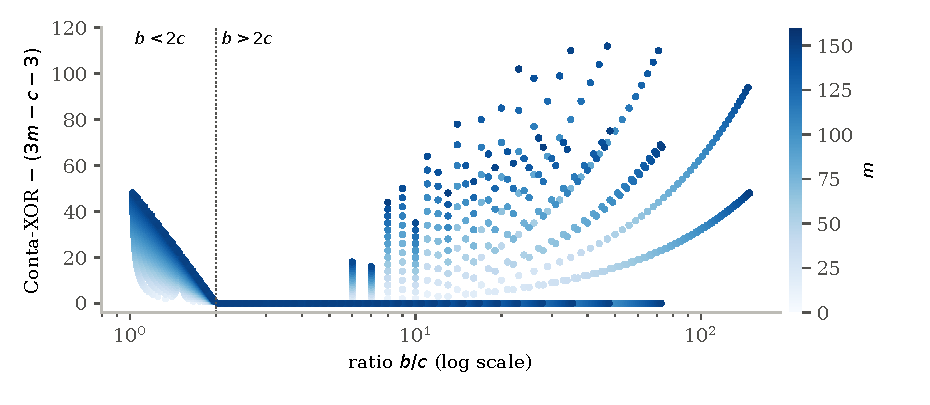
\includegraphics[width=\textwidth]{fig_gain.pdf}
\caption{\ours{} Greedy count minus closed form, $\CX(f)-(3m-c-3)$, for the $3\,541$
generic members with $m\le150$. The difference is never negative. Left of $b/c=2$ it
equals $2c-b$; between $2$ and $6$ it is zero; for larger ratios the greedy algorithm
loses gates on members with small $c$.}
\label{fig:gain}
\end{figure}

\begin{table}[t]
\centering\small
\caption{\ours{} Irreducible members of the second family at the NIST degrees. ``Thesis''
marks the values published in \cite[Tab.~17]{Banegas2015}.}
\label{tab:thesis}
\begin{tabular}{@{}r l r r r r r r@{}}
\toprule
$m$ & $f$ & $b$ & $c$ & $\dX$ & $\CX$ & $3m-c-3$ & depth\\
\midrule
163 & $x^{163}+x^{117}+x^{71}+x^{46}+1$ & 71 & 46 & 649 & 461 & \textbf{440} & 4\\
233 & $x^{233}+x^{158}+x^{83}+x^{75}+1$ & 83 & 75 & 866 & 688 & \textbf{621} & 4\\
233 & $x^{233}+x^{217}+x^{201}+x^{16}+1$ & 201 & 16 & 1687 & 680 & 680 & 7\\
409 & $x^{409}+x^{294}+x^{179}+x^{115}+1$ & 179 & 115 & 1642 & 1160 & \textbf{1109} & 4\\
409 & $x^{409}+x^{337}+x^{265}+x^{72}+1$ & 265 & 72 & 1823 & 1152 & 1152 & 4\\
571 & $x^{571}+x^{389}+x^{207}+x^{182}+1$ & 207 & 182 & 2145 & 1685 (thesis) & \textbf{1528} & 4\\
571 & $x^{571}+x^{465}+x^{359}+x^{106}+1$ & 359 & 106 & 2531 & 1604 (thesis) & 1604 & 4\\
571 & $x^{571}+x^{549}+x^{527}+x^{22}+1$ & 527 & 22 & 6297 & 1688 (thesis) & 1688 & 11\\
\bottomrule
\end{tabular}
\end{table}

\paragraph{Small degrees.}
For the generic members of degrees $9$ and $10$, $f_{5,2}$ and $f_{4,3}$, the
Boyar--Peralta heuristic \cite{BoyarPeralta2010}, which may use cancellations (best of
$10$ runs), finds programs of lengths $22$ and $24$, equal to $3m-c-3$; the greedy counts
are $22$ and $26$. For the smallest member $f_{3,2}$ (degree $7$, special) both the
closed form and Boyar--Peralta give $16$, one less than the greedy count.

% ==================================================================
\section{Comparison with the first family and with other polynomials}\label{sec:comparison}
% ==================================================================

\paragraph{Choosing $c$.}
By \cref{thm:main} the cost decreases with $c$. Since $c\le\lfloor(m-1)/3\rfloor$, the
best possible generic member has cost close to $3m-\tfrac m3=\tfrac83m$. For the first
family the cost $3m-2$ does not depend on $(b,c)$, except in the special case $m=5c$.

\paragraph{Census.}
We tested the irreducibility of all members of both families and of all trinomials for
$5\le m\le1100$, using Rabin's test \cite{Rabin1980}. \Cref{tab:census} summarises the
result, and \cref{fig:census} shows, for the degrees without irreducible trinomials,
the cost per bit of the best member of each family.

\begin{table}[t]
\centering\small
\caption{\ours{} Census for $5\le m\le1100$ ($1\,096$ degrees). ``Best'' uses
\cref{thm:main} for the second family, $3m-2$ or $\tfrac{12}{5}m-1$ for the first family
\cite{BCP2019}, and $\tfrac74m-1$ for equally spaced members.}
\label{tab:census}
\begin{tabular}{@{}l r@{}}
\toprule
irreducible members of the second family & $1\,508$\\
degrees with at least one member: second family / first family & $720$ / $502$\\
degrees with members of both families & $405$\\
\quad of which the second family is cheaper & $403$ (mean saving $7.3\%$)\\
\quad of which the first family is cheaper / tie & $1$ ($m=155$) / $1$ ($m=5$)\\
degrees without irreducible trinomials & $502$\\
\quad covered by the second family / by the first family & $288$ / $229$\\
\quad covered by the second family only & $112$\\
\quad covered by neither & $161$\\
mean cost per bit of the best generic member of the second family & $2.77$\\
\bottomrule
\end{tabular}
\end{table}

\begin{figure}[t]
\centering
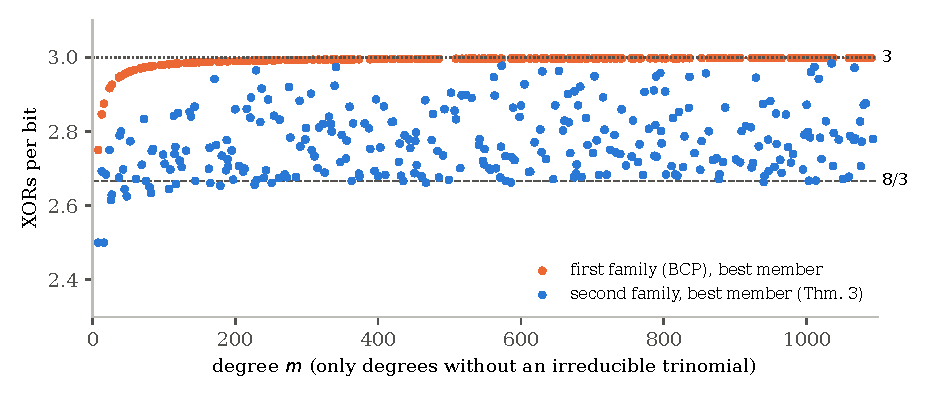
\includegraphics[width=\textwidth]{fig_census.pdf}
\caption{\ours{} Best reduction cost per bit, for the degrees $m\le1100$ without
irreducible trinomials, of the best member of the first family (BCP) and of the second
family (\cref{thm:main}). The dashed line is the asymptotic limit $\tfrac83$ of the second
family.}
\label{fig:census}
\end{figure}

The only degree in which the first family wins is $m=155$, where its member with $b=2c$
reaches $\tfrac{12}{5}m-1=371$ and the best generic member of the second family needs
$411$. Degrees $\equiv0\pmod8$ deserve a comment, since they never have irreducible
trinomials; the second family has members in $25$ of them, for instance
$x^{16}+x^{11}+x^6+x^5+1$ (\cref{ex:16}), $x^{48}+x^{33}+x^{18}+x^{15}+1$ ($126$ XORs) and
$x^{144}+x^{99}+x^{54}+x^{45}+1$ ($384$ XORs).

\paragraph{NIST degrees.}
\Cref{tab:nist} compares the best members of both families at the NIST degrees with the
NIST polynomials and with trinomials where they exist. At $m=163$ and $m=571$, where no
irreducible trinomial exists, the second family reduces with $22.9\%$ and $23.7\%$ fewer
XORs than the NIST pentanomials (as counted by Conta-XOR) and $9.7\%$ and $10.7\%$ fewer
than the first family. At $m=283$ the second family has no irreducible member. At $233$
and $409$ trinomials are cheaper, as expected.

\begin{table}[t]
\centering\small
\caption{\ours{} Best known reduction costs at the NIST degrees. NIST pentanomials: Conta-XOR
counts from \cite{Banegas2015}; first family: \cite{BCP2019}; second family:
\cref{thm:main}.}
\label{tab:nist}
\begin{tabular}{@{}r r r r r@{}}
\toprule
$m$ & NIST polynomial & trinomial & first family & second family\\
\midrule
163 & 571 & -- & 487 & \textbf{440}\\
233 & 464 (trinomial) & \textbf{464} & 697 & 621\\
283 & 862 & -- & \textbf{847} & --\\
409 & 816 (trinomial) & \textbf{816} & -- & 1109\\
571 & 2003 & -- & 1711 & \textbf{1528}\\
\bottomrule
\end{tabular}
\end{table}

% ==================================================================
\section{Discussion and conclusion}\label{sec:conclusion}
% ==================================================================

\paragraph{Why the second family was hard.}
For the first family, $x^m\equiv(x^b+1)(x^c+1)$ and $m=2b+c$ make the high part fold
into the low part after a bounded number of steps. For the second family the quotient
has long-range dependencies of stride $3c$, visible only after solving the recurrence
\eqref{eq:rec}. The greedy counter captures part of this structure, and it reaches the
optimum of our construction when $2c<b<6c$, but it misses the sharing across the comb sums
when $b<2c$ and loses track of the long combs when $b\gg c$. This explains the remark in
the thesis that the family required ``a greater understanding of the reduction process''.

\paragraph{What the closed form gives.}
The program of \cref{alg:main} is uniform, easy to generate for any $(b,c)$, has small
depth when $b\le4c+1$, and its cost depends on the parameters only through $m$ and $c$.
It turns the second family into a practical alternative wherever it has irreducible
members, and in particular in degrees without trinomials.

\paragraph{Limitations and open questions.}
(i) \Cref{thm:main} is an upper bound. For the generic members with $m\le10$ it
matches the Boyar--Peralta heuristic, but lower bounds for larger degrees are open.
(ii) Special members, of the form $G(x^g)$ with a short $G$, can be reduced with fewer
gates; a uniform treatment of these cases is left open. (iii) The irreducibility of the
members is still characterised only computationally. (iv) Joint optimisation of the
product and the reduction, as in Mastrovito-type multipliers
\cite{Mastrovito1989,ReyhaniHasan2004}, and area--delay trade-offs remain to be studied.

\paragraph{Reproducibility.}
The generator of \cref{alg:main} with symbolic verification, the irreducibility census
and the scripts that produced the tables and figures are available from the authors and
will be published with the final version.

\printbibliography
\end{document}
